\documentclass[10pt, conference]{IEEEtran}
\usepackage[english]{babel}
\usepackage[T1]{fontenc}
\usepackage[usenames]{color}
\usepackage{colortbl}
\usepackage{comment}
\usepackage{graphicx}
\usepackage{array, colortbl}
\usepackage{multirow}
\usepackage{booktabs}
\usepackage{float}
\usepackage[obeyspaces,hyphens,spaces]{url}
\usepackage{balance}
\usepackage[normalem]{ulem}
\usepackage{xspace}
\usepackage{microtype}
\usepackage{pgfgantt}
\pagenumbering{arabic}
\pagestyle{empty}
\clubpenalty = 10000
\widowpenalty = 10000
\displaywidowpenalty = 10000
\usepackage{cleveref}
\crefname{figure}{Fig.}{Figs.}

\makeatletter
\renewcommand{\paragraph}[1]{\noindent\textbf{#1}.}
\makeatother

% Every number below is a macro generated from results/numbers.json by src/make_macros.py.
% Generated by src/make_macros.py from results/numbers.json. Do not edit by hand.
\newcommand{\ciFossil}{[19.3, 19.9]\%\xspace}
\newcommand{\ciNeverRevised}{[62.4, 63.1]\%\xspace}
\newcommand{\ciPlaceholder}{[28.9, 29.6]\%\xspace}
\newcommand{\numArchivePlaceholder}{19{,}651\xspace}
\newcommand{\numArchived}{156{,}372\xspace}
\newcommand{\numCohortCommits}{735{,}667\xspace}
\newcommand{\numCohortSpecs}{468{,}163\xspace}
\newcommand{\numCommitTable}{780{,}335\xspace}
\newcommand{\numDelta}{41{,}582\xspace}
\newcommand{\numDroppedSpecs}{2{,}632\xspace}
\newcommand{\numFlagOnly}{1{,}674\xspace}
\newcommand{\numFossilRepos}{2{,}488\xspace}
\newcommand{\numFossils}{14{,}294\xspace}
\newcommand{\numFossilsArchiveText}{13{,}426\xspace}
\newcommand{\numLiving}{72{,}971\xspace}
\newcommand{\numLivingOldNinety}{26{,}887\xspace}
\newcommand{\numLivingRepos}{6{,}085\xspace}
\newcommand{\numLivingYoungThirty}{16{,}099\xspace}
\newcommand{\numNoBoth}{1{,}329\xspace}
\newcommand{\numNoContent}{2{,}488\xspace}
\newcommand{\numNoHistory}{1{,}473\xspace}
\newcommand{\numOpenSpecFiles}{274{,}955\xspace}
\newcommand{\numOpenSpecRepos}{8{,}926\xspace}
\newcommand{\numOrphanCommits}{41{,}170\xspace}
\newcommand{\numPlaceholderRevised}{7{,}031\xspace}
\newcommand{\numRenameChecked}{30\xspace}
\newcommand{\numRenameLivingChecked}{15\xspace}
\newcommand{\numRenameLivingTrue}{1\xspace}
\newcommand{\numRenamePlainMatch}{29\xspace}
\newcommand{\numRepoK}{3\xspace}
\newcommand{\numRepos}{73{,}030\xspace}
\newcommand{\numReposK}{4{,}618\xspace}
\newcommand{\numRevised}{27{,}184\xspace}
\newcommand{\numSampleFossils}{375\xspace}
\newcommand{\numSampleFossilsTen}{96\xspace}
\newcommand{\numSampleRevised}{379\xspace}
\newcommand{\numSampleRevisedTen}{96\xspace}
\newcommand{\numSpecFiles}{470{,}795\xspace}
\newcommand{\pctArchivedNeverRevised}{96.7\%\xspace}
\newcommand{\pctConfSample}{95\%\xspace}
\newcommand{\pctDeltaNeverRevised}{89.7\%\xspace}
\newcommand{\pctFlagPrecision}{92.2\%\xspace}
\newcommand{\pctFlagPurposeTbd}{98.7\%\xspace}
\newcommand{\pctFlagRecall}{100.0\%\xspace}
\newcommand{\pctFossil}{19.6\%\xspace}
\newcommand{\pctFossilOldNinety}{16.8\%\xspace}
\newcommand{\pctLivingYoungNinety}{63\%\xspace}
\newcommand{\pctLivingYoungThirty}{22\%\xspace}
\newcommand{\pctNeverRevised}{62.7\%\xspace}
\newcommand{\pctNeverRevisedOldNinety}{58.0\%\xspace}
\newcommand{\pctNoPlaceholder}{70.8\%\xspace}
\newcommand{\pctOpenSpecFiles}{58.4\%\xspace}
\newcommand{\pctPlaceholder}{29.2\%\xspace}
\newcommand{\pctPlaceholderRevised}{9.6\%\xspace}
\newcommand{\pctReposAllFossil}{7\%\xspace}
\newcommand{\pctReposExtreme}{70\%\xspace}
\newcommand{\pctReposZeroFossil}{56\%\xspace}
\newcommand{\pctTopFossilRepo}{0.94\%\xspace}

\newcommand{\fp}[1]{\texttt{#1}}

\title{The Myth of the ``Living'' Document:\\Are OpenSpec's Living Specifications Ever Revised?}
% TODO(team): add e-mail addresses.
\author{\IEEEauthorblockN{Tran Vo \quad Thanh Nghiep Quan}
\IEEEauthorblockA{\emph{Dep. of Computer and Software Engineering, Polytechnique Montr\'eal}, Montr\'eal, Canada}}

\begin{document}
\maketitle

\begin{abstract}
In spec-driven development (SDD), developers describe what to build in a Markdown
specification and an AI coding agent implements it. OpenSpec, the SDD tool with the most
spec files in SpecMine (the MSR 2027 Mining Challenge dataset), keeps one \emph{living} spec
per capability and calls these specs the source of truth for how the system currently behaves.
We ask whether living specs are actually maintained. In a preliminary analysis of
\numLiving living specs, \pctNeverRevised were never revised after creation, and
\pctFossil (\numFossils specs) are \emph{fossils}: they still hold a TBD placeholder in
their Purpose section, usually the one OpenSpec's archive step writes, and nobody ever
edited them.
We propose three research questions on revision behaviour, fossil prevalence and
characterization, and cross-tool comparison.
\end{abstract}

\section{Problem Statement}
\label{sec:statement}

SDD tools such as OpenSpec~\cite{openspec} and GitHub Spec Kit~\cite{speckit} make the
specification the input of AI coding agents~\cite{boeckeler2025}. In OpenSpec, a developer
proposes a change (\fp{changes/<name>/} with a proposal, delta specs, a design and tasks),
the agent implements it, and \emph{archiving} moves the change to \fp{changes/archive/}
and merges its delta specs into \fp{openspec/specs/}. OpenSpec's documentation states that
these specs are the source of truth: they describe how your system currently
behaves~\cite{openspec}, and agents read them as context for every later change. A spec
that stops changing while the code moves on is wrong input for the next agent.

OpenSpec gives us an unusual marker of unfinished documentation. Before v1.7.0, archiving a
change that introduced a new capability always wrote
``\texttt{TBD - created by archiving change <name>. Update Purpose after archive.}'' into the
new spec's Purpose section~\cite{openspec_pr1431}. The fix (PR~\#1431) was released on
July 29, 2026, after SpecMine's crawl ended (July 11, 2026), so every spec in the snapshot
was created by tool versions that could write the placeholder. A spec that still holds it,
and was never revised, was written once and forgotten.

Outdated documentation is a long-standing problem~\cite{lethbridge2003,aghajani2019,tan2024}.
The SpecMine authors list spec lifecycle, including ``placeholders never filled,'' as an
open question~\cite{specmine_paper}. Their practitioners report \emph{spec decay} in living
specs, but commit counts alone cannot show it~\cite{specmine_paper}; we add a
tool-written marker.

\paragraph{Link with the course} Living specs are configuration for AI agents,
kept as code next to the system they describe. Their staleness mirrors configuration drift
in DevOps. OpenSpec has since added a validation check for the
placeholder~\cite{openspec_pr1671}, a gate a CI pipeline can enforce; we measure how much
such gates are needed.

\section{Research Questions}
\label{sec:research-idea}

All analyses start from \emph{commits per spec file}. A \emph{revision} is a
commit that touches the file after its creation commit. A \emph{fossil} is a living spec
whose snapshot content holds an unfilled placeholder and that has zero revisions.

\textbf{RQ1: Do living specs get revised?} \emph{Motivation:} if living specs are the
source of truth, each archived change that touches a capability should revise its spec.
\emph{Approach:} distribution of revisions per living spec, compared with archived specs
(frozen by design; the reference), delta specs, and Spec Kit specs; Wilson 95\% CIs for
proportions and $\chi^2$ tests with Cram\'er's~$V$. If time permits, a Kaplan--Meier curve of time to first
revision handles specs too young to have been revised yet.

\textbf{RQ2: How prevalent are fossil living specs, and what kinds of specs become
fossils?} \emph{Motivation:} the naive ``never revised'' rate mixes finished specs with
forgotten ones; the placeholder helps tell them apart. \emph{Approach:} we first measure
how common fossils are. We report their share of living specs with CIs, split into fossils,
specs whose placeholder survived a revision, and specs without a placeholder, and compare
it with the naive measure and a no-placeholder control group. We then ask what fossils look
like, as the instructor suggested. After computing the fossil rate of each repository, we
sample fossils and, for contrast, \emph{fixed} specs, whose first version had the
placeholder and whose snapshot does not (found with \texttt{git log -p} on cloned
repositories), at most one per repository, with a fixed seed. Each sampled spec gets
automatic features (repository activity, bulk creation, spec size, later code
changes and, for fixed specs, whether a human, an agent or a bulk update filled the
placeholder) and a category from manual coding: both students open-code 30 specs to build a
codebook, then double-code 100 specs (Cohen's $\kappa$). An LLM, run at temperature~0 and
tuned on the pilot set only, labels the remaining sample of about 375 fossils if it reaches
$\kappa \geq 0.6$ on held-out human labels.

\textbf{RQ3: Is write-once the same across tools?} \emph{Motivation:} tools label spec
files differently, and only OpenSpec encodes lifecycle roles~\cite{specmine_paper}. A pooled
comparison mixes in archived specs, whose history restarts at the archive move
(\pctArchivedNeverRevised have no revision). \emph{Approach:} compare tools after
removing archived specs, and contrast with the pooled comparison.

\paragraph{Robustness} File age: \pctLivingYoungThirty of living specs were created less
than 30 days before the snapshot, so we re-run every result without specs younger than
30, 60 and 90 days (for specs at least 90 days old, \pctNeverRevisedOldNinety were never
revised and \pctFossilOldNinety are fossils). Repository dominance: per-repository caps and
leave-largest-out. Inactive repositories separate forgotten from finished specs.

\section{Dataset}
\label{sec:dataset}
\sloppy

We use SpecMine v1.0 (July 2026 snapshot)~\cite{specmine_dataset,specmine_paper}:
\numSpecFiles spec files from \numRepos GitHub repositories. OpenSpec accounts for
\numOpenSpecFiles files (\pctOpenSpecFiles) in \numOpenSpecRepos repositories. We query the
Parquet tables with DuckDB: \texttt{spec\_files} (tool, lifecycle role),
\texttt{spec\_file\_commits} (per-file history) and \texttt{spec\_content\_features} (the
placeholder flag), plus the snapshot text of every spec (\texttt{specs.jsonl.gz}, on Zenodo
only). Our cohort keeps the \numCohortSpecs
specs with both a fetched commit history and fetched content (\numCohortCommits commits);
the \numDroppedSpecs excluded files lack history (\numNoHistory), content (\numNoContent), or
both (\numNoBoth). \Cref{tab:prelim} gives our preliminary numbers. \Cref{fig:repo} shows that fossils cluster by repository:
\pctReposExtreme of repositories with at least \numRepoK living specs have a fossil rate
at or below 10\% or at or above 90\%, so we sample fossils per repository.

\begin{figure}[t]
\centering
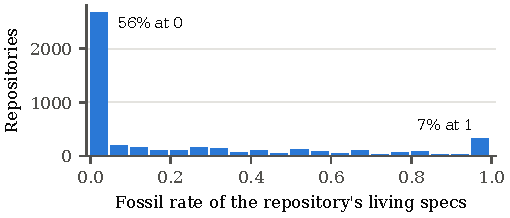
\includegraphics[width=\columnwidth]{../results/figures/repo_fossil_rate.pdf}
\caption{Fossil rate per repository ($\geq$\numRepoK living specs; \numReposK repositories).}
\label{fig:repo}
\end{figure}

\begin{table}[t]
\centering
\caption{Preliminary results for OpenSpec living specs}
\label{tab:prelim}
\footnotesize
\begin{tabular}{@{}lrr@{}}
\toprule
Quantity & Value & 95\% CI \\
\midrule
Living / delta / archived specs & \multicolumn{2}{r@{}}{\numLiving\,/\,\numDelta\,/\,\numArchived} \\
Living specs never revised & \pctNeverRevised & \ciNeverRevised \\
Unfilled placeholder & \pctPlaceholder & \ciPlaceholder \\
\quad and never revised (fossil) & \pctFossil & \ciFossil \\
\quad and revised at least once & \pctPlaceholderRevised & \\
Repos holding fossils (largest: \pctTopFossilRepo) & \numFossilRepos & \\
\bottomrule
\end{tabular}
\end{table}

\paragraph{Data caveats we already checked} (1)~SpecMine histories do not follow renames.
In \numRenamePlainMatch of \numRenameChecked sampled specs, SpecMine's commit count equals a
path-only \texttt{git log}; \numRenameLivingTrue of \numRenameLivingChecked living specs was renamed. Revision counts are therefore lower bounds. (2)~The placeholder flag describes the snapshot only. It flags all \numArchivePlaceholder
specs holding the archive placeholder text (recall \pctFlagRecall); \pctFlagPrecision of
flagged specs hold that text and \pctFlagPurposeTbd have some TBD Purpose. (3)~SpecMine has no code commits outside its pull-request layer, so
code activity and fixed specs require cloning repositories.

\section{Related Work}
\label{sec:related}

\paragraph{SDD and SpecMine} Agarwal et al.~\cite{specmine_paper} release SpecMine and study
SDD through practitioner interviews and 266 repositories. They report that living specs
decay but do not measure it at scale. We answer their lifecycle question with per-file
history over all \numLiving OpenSpec living specs.

\paragraph{Outdated documentation} Lethbridge et al.~\cite{lethbridge2003} found that
software documentation is often out of date, and Aghajani et al.~\cite{aghajani2019} include
up-to-dateness in their taxonomy of documentation issues. Tan et al.~\cite{tan2024} detect
outdated code references in README and wiki files; we study specs the tool labels current.

\paragraph{Self-admitted technical debt} Potdar and Shihab~\cite{potdar2014} and Bavota and
Russo~\cite{bavota2016} study debt that developers admit in code comments and whether it is
removed. In our setting the tool writes the debt marker, and we ask whether anyone pays it.

\section{Time Planning of Project}
\label{sec:schedule}
\Cref{fig:gantt} shows the plan.

\begin{figure}[h]
\centering
\footnotesize
\begin{ganttchart}[hgrid, vgrid, x unit=0.42cm, y unit chart=0.30cm,
  bar height=0.55, bar/.append style={fill=black!35, draw=black!70},
  title height=0.9, title label font=\scriptsize, bar label font=\scriptsize]{1}{11}
\gantttitlelist{1,...,11}{1} \\
\ganttbar{Explore data, proposal}{1}{2} \\
\ganttbar{RQ1, RQ3}{3}{4} \\
\ganttbar{RQ2; codebook v1}{5}{6} \\
\ganttbar{Double coding; LLM}{7}{7} \\
\ganttbar{Stats, robustness}{8}{8} \\
\ganttbar{Report, presentation}{9}{11}
\end{ganttchart}
\caption{Schedule by week (week 1 starts Sep.~28, 2026; the report is due Dec.~18).}
\label{fig:gantt}
\end{figure}

\balance
\bibliographystyle{IEEEtran}
\bibliography{proposal.bib}
\end{document}
